\begin{frame}{Experiment 1}
\setbeamercovered{invisible}
\fontsize{12pt}{15}\selectfont
\only<1-2>{{\large\textbf{Results:}}}
\only<1>{\begin{figure}
    \centering
    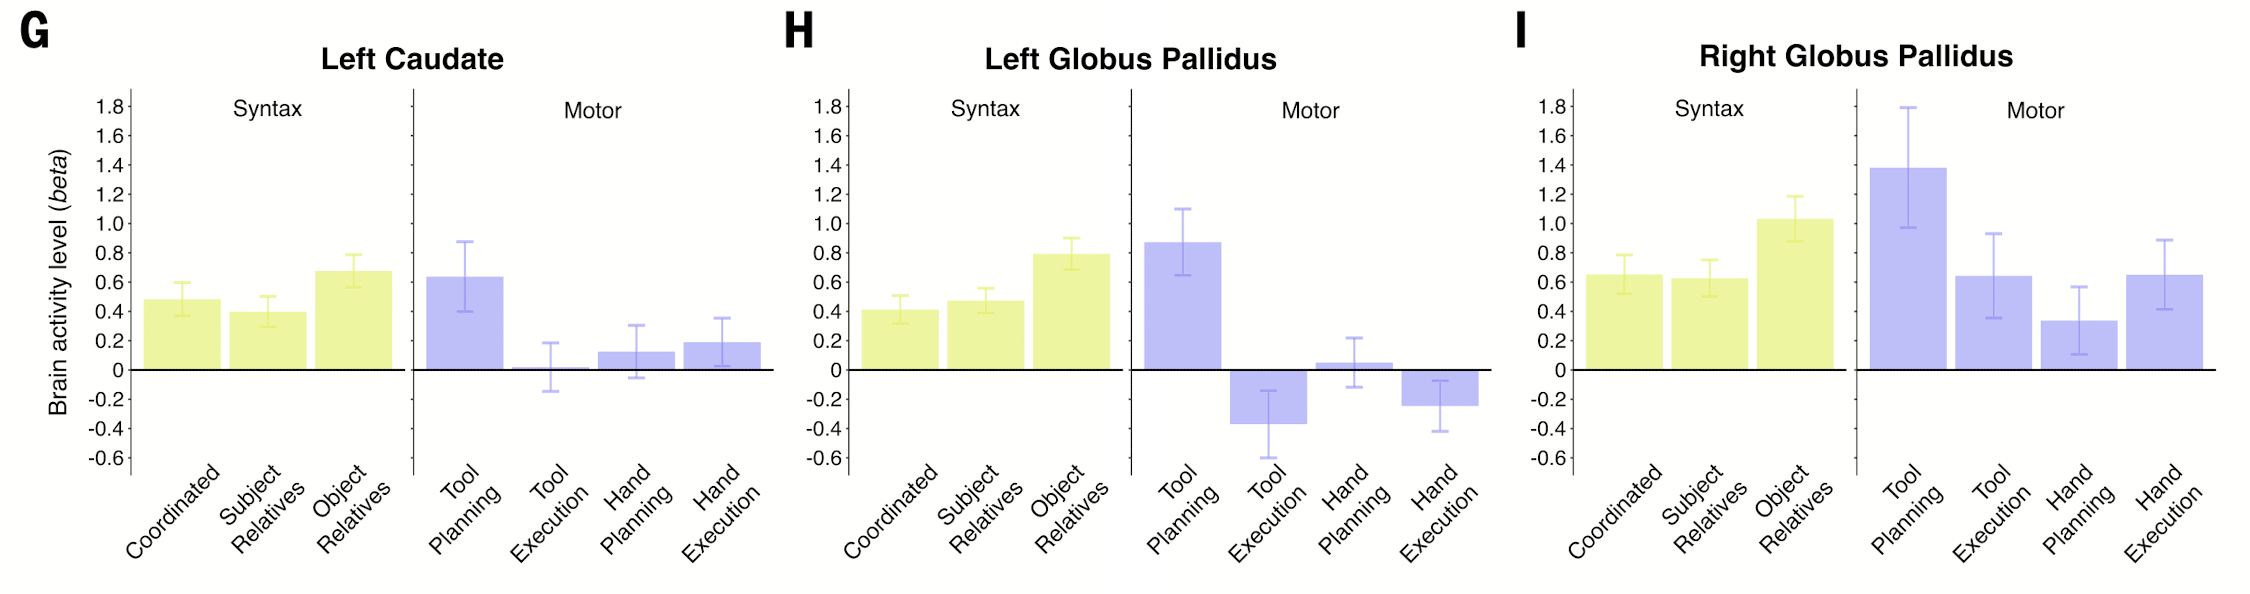
\includegraphics[width=10.5cm]{images/paper_pics/fig1GHI.png}
    \caption*{Syntactic and tool-use planning shared significant activations of the left caudate nucleus (lCau) and bilateral GPi}
    \label{fig:label4}
\end{figure}
}
\pause
\only<2>{
\begin{itemize}
\item Both networks anatomically \textbf{overlapped} within the \textbf{BG}
\item Clusters found in proximity of left IFG did not overlap
\item \textbf{No} significant \textbf{shared} activation for \textbf{syntax} and \textbf{free-hand planning}
\end{itemize}}
\pause

\only<3>{{\large \textbf{To \textbf{rule out} contribution of \textbf{working memory} to this overlap}\\
\begin{itemize}
    \item Measured brain activity while same participants performed two verbal \textbf{n-back tasks}
    \item \textbf{Did not} significantly \textbf{overlap} with tool-use planning network
\end{itemize}}}

\end{frame}